\documentclass{article}
\usepackage{graphicx}
\usepackage{amsmath}

\title{Object-Oriented Programming Concepts for Beginners: What is Inheritance?}
\author{Your Name}
\date{\today}

\begin{document}

    \section{first}

    Inheritance is one of the core concepts of object-oriented programming (OOP) languages. It is a mechanism where you can to derive a class from another class for a hierarchy of classes that share a set of attributes and methods.

    You can use it to declare different kinds of exceptions, add custom logic to existing frameworks, and even map your domain model to a database.
    Try Stackify’s free code profiler, Prefix, to write better code on your workstation. Prefix works with .NET, Java, PHP, Node.js, Ruby, and Python.
    \begin{figure}[h]
        \begin{minipage}[t]{0.48\linewidth}
            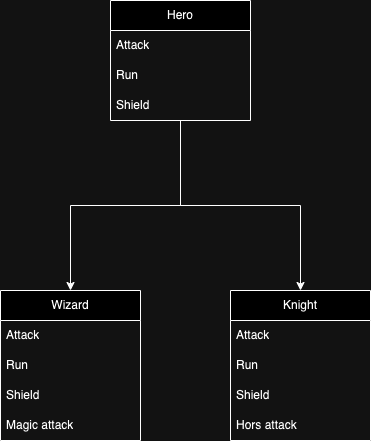
\includegraphics[width=\textwidth]{test}
        \end{minipage}
        \hfill
        \begin{minipage}[t]{0.48\linewidth}
            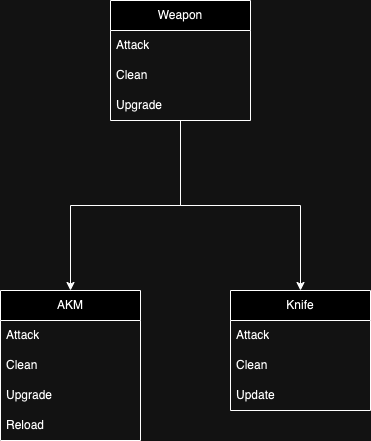
\includegraphics[width=\textwidth]{second}
        \end{minipage}
        \caption{Exemple.}
        \label{fig:my_image}
    \end{figure}

    \section*{Matrix Example}
    Here is a 5x5 matrix:
    \[
        \begin{bmatrix}
            1 & 2 & 3 & 4 & 5 \\
            6 & 7 & 8 & 9 & 10 \\
            11 & 12 & 13 & 14 & 15 \\
            16 & 17 & 18 & 19 & 20 \\
            21 & 22 & 23 & 24 & 25 \\
            \end{bmatrix}
    \]

    The sum of the first $n$ natural numbers:
    \[
        \sum_{k=1}^{n} k = 1 + 2 + 3 + \ldots + n
    \]
    \[
        \lim_{{x \to \infty}} \frac{1}{x} = 0
    \]


\end{document}
